\documentclass[11pt,a4paper]{article}
\usepackage[utf8]{inputenc}
\usepackage[english]{babel}
\usepackage{amsmath}
\usepackage{amsfonts}
\usepackage{amssymb}
\usepackage{graphicx}
\usepackage[left=2cm,right=2cm,top=2cm,bottom=2cm]{geometry}
\begin{document}

\begin{flushright}
Longitudinal Analysis 2021

Homework 2

Ian Arriaga MacKenzie
\end{flushright}

\textbf{Question 1}\\

Fitting both a linear regression model and superimposing the PCA calculated slope over the original data yields the following plot:

\begin{center}
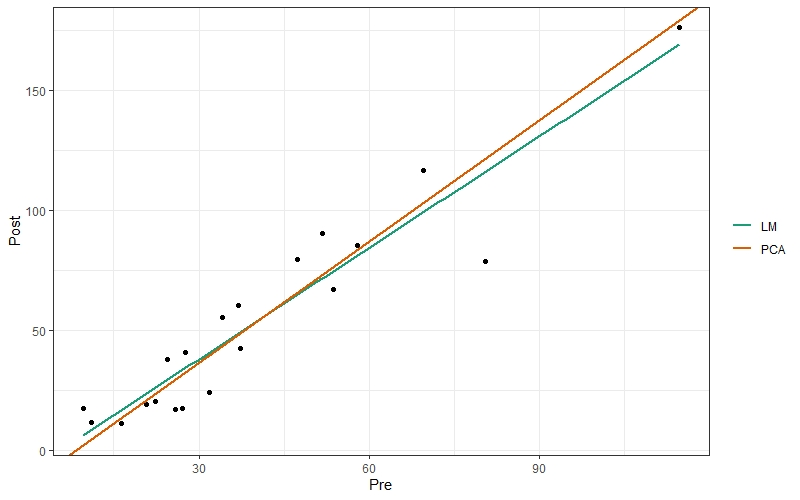
\includegraphics[scale=0.7]{pca_plot.jpeg}
\end{center}

The slopes are very close, with the PCA slope: 1.684 and LM slope: 1.546.\\

\textbf{Question 2}\\

\textit{(a)}\\

The main difference between a general linear model and a linear mixed model is the inclusion of the vector and design matrix (generally denoted \textbf{\textit{Zu}}) which define the random effects of the LMM. The unknown random effects \textbf{\textit{u}} generally corresponds to random intercepts or slopes for mixed effects models, and are defined by the variance-covariance matrix \textbf{\textit{G}}. The \textbf{\textit{Z}} matrix is usually an identity matrix with dimensions of the number of random effects in the model.\\

\textit{(b)}\\

The profile likelihood is a re-expression of the standard likelihood in which all other parameters are chosen specifically to maximize the parameter of interest. This is generally done through an EM algorithm to sequentially step through the parameter space in order to find the optimal solution, and is used to identify estimates for single parameters. The restricted likelihood optimizes the likelihood of the full residuals, which in turn allows the random effects to be estimated without bias.\\

\textit{(c)}\\

Unable to complete.\\

\textbf{Question 3}\\

\textit{(a)}\\

Using a wald-type test, we return a p-value of 0.749 which suggests there is no interaction over time for the 30 and 60mg BASF groups over the 5 time points.\\

\textit{(b)}\\

Again, using a wald-type test, we return a p-value of 1.32E-10 which now does suggest there is difference between baseline and 12 weeks across all 4 groups.\\

\textit{(c)}\\

Fitting a cubic model with continuous time is almost like fitting the categorical time model however it is one degree short and therefor would probably result in higher variance in the residuals. With 5 time points, a polynomial of degree 4 would be needed to fit the data "perfectly" and so a cubic polynomial for time would be good but not great.\\

\textit{(d)}\\

Modeling \textit{Time0} as a covariate value is somewhat analagous to having a random intercept model. Instead of actually having random intercepts based on subject, each subject would have a different intercept based linearly on their starting carotene levels.\\

\textit{(e)}\\

The polynomial estimates are, linear: 479.68, quadratic: -216.34, cubic: 90.69.\\

\textbf{Question 4}\\

Unable to complete.

\newpage
\textbf{R Code Appendix}

\begin{verbatim}
# Longitudinal Analysis
# Homework 2 - Ian Arriaga MacKenzie

# load libraries
library(tidyverse)
library(ggfortify)
library(RColorBrewer)
library(lme4)
library(lmerTest)
library(emmeans)

#### Q1

# load eNO data
eno_df = read.csv("~/GitHub/BIOS6643Longitudinal/homework2/eno_data.txt", sep="") %>% 
  rename(pre = eno_pre,
         post = eno_post)

# set colorblind colors
colpallet = brewer.pal(8, "Dark2")
colval = c("LM" = colpallet[1], "PCA" = colpallet[2])

# PCA
eno_pca = prcomp(eno_df)

# pca slope
pca_slope = eno_pca$rotation[2,1]/eno_pca$rotation[1,1]
# eno pre/post mean
mp = c(mean(eno_df$pre), mean(eno_df$post))
# y intercept using pca slope and passing through mean
yint = pca_slope * (0 - mp[1]) + mp[2]

# Slope information
lm(formula = post ~ pre,
   data = eno_df)

# Plot LM and PCA slope over data
ggplot(eno_df, aes(pre, post))+
  geom_point() +
  geom_smooth(aes(color = "LM"),
              method = "lm", 
              formula = y ~ x,
              se = F,
              size = 1) +
  geom_abline(color = colval[2],
              slope = pca_slope,
              intercept = yint,
              size = 1) +
  theme_bw() +
  labs(x = "Pre",
       y = "Post") +
  scale_colour_manual(name = element_blank(),
                      values = colval, 
                      guide = guide_legend(override.aes = aes(fill = NA)))
  
#### Q2

# Read data
bc_df = read.csv("~/GitHub/BIOS6643Longitudinal/homework2/beta_carotene_univar.csv")

# Clean data
bc_cl = bc_df %>% 
  rename(group = Prepar,
         id = Id,
         carotene = y,
         time = time) %>% 
  mutate(group_fac = factor(group,
                            levels = c(1,2,3,4),
                            labels = c("Solatene_30mg",
                                       "Roche_60mg",
                                       "BASF_30mg",
                                       "BASF_60mg")),
         time_fac = factor(time,
                           levels = c(0,6,8,10,12),
                           labels = c("0_m", "6_m", "8_m", "10_m", "12_m")))


# fit LMER
bc_fit = lmer(formula = carotene ~ group_fac + time_fac + group_fac*time_fac + (1 | id) - 1,
              data = bc_cl)
summary(bc_fit)
anova(bc_fit)

# extract coef/var
coef_fit = fixef(bc_fit)
var_fit = vcov(bc_fit)

# Part A
waldmat = matrix(c(0, 0, 0, 0, 0, 0, 0, 0, 0, 1, 1, 0, 0, 0, 0, 0, 0, 0, 0, 0,
                   0, 0, 0, 0, 0, 0, 0, 0, 0, 0, 0, 0, 1, 1, 0, 0, 0, 0, 0, 0,
                   0, 0, 0, 0, 0, 0, 0, 0, 0, 0, 0, 0, 0, 0, 0, 1, 1, 0, 0, 0,
                   0, 0, 0, 0, 0, 0, 0, 0, 0, 0, 0, 0, 0, 0, 0, 0, 0, 0, 1, 1), byrow = T, 4, 20)

wald2 = waldmat %*% coef_fit
chival = t(wald2) %*% solve(waldmat %*% var_fit %*% t(waldmat)) %*% wald2
pchisq(as.numeric(chival), 8, lower.tail = F)

# Part B
waldmat = matrix(c(1, 1, 1, 1, 0, 0, 0, 0, 0, 0, 0, 0, 0, 0, 0, 0, 0, 0, 0, 0,
                   1, 1, 1, 1, 0, 0, 0, 1, 0, 0, 0, 0, 0, 0, 0, 0, 0, 1, 1, 1), byrow = T, 2, 20)

wald2 = waldmat %*% coef_fit
chival = t(wald2) %*% solve(waldmat %*% var_fit %*% t(waldmat)) %*% wald2
pchisq(as.numeric(chival), 4, lower.tail = F)

# Part E
bc_polyfit = lmer(formula = carotene ~ group_fac + poly(time, 3) + group_fac*time + (1 | id) - 1,
                  data = bc_cl)

summary(bc_polyfit)
\end{verbatim}

\end{document}